\documentclass[12pt]{article}
\usepackage{amsmath}
\usepackage{graphicx}
\usepackage[utf8]{inputenc}

\title{Pendulul Invers}
\author{Gengiu Robert-Constantin}
\begin{document}
\maketitle
\flushleft
Introducere \newline
Pendulul Invers este o problema clasica de dinamica nonliniara si de control. Scopul final este de a stabiliza pendulul, astfel incat sa faca unghi nul cu verticala. Pornind de la modelul matematic, se obtin ecuatiile de miscare, care vor fi liniarizate, si in final se va calcula un tip de controler cu ajutorul Matlab-ului. Mai departe, avand toate acestea calculate, se poate realiza o simulare grafica a sistemului.\newline 

\center
~~~~~~~~~~~Prezentarea pe scurt a modelului matematic\newline
\begin{center}
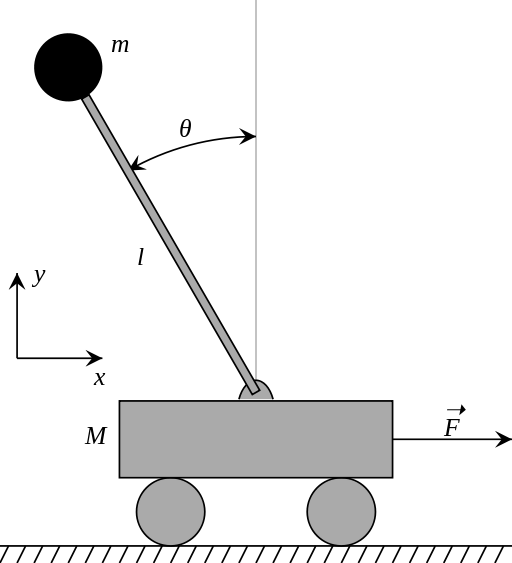
\includegraphics[width = 0.4\textwidth]{pen.png} \newline 
\end{center}
\flushleft

\medskip
\begin{center}
  \begin{tabular}{ | l | r | }
    \hline
    Variabila & Definitie \\  \hline
    M & Masa cartului(kg) \\ \hline
    m & Masa pendulului(kg) \\ \hline
     x & Deplasarea cartului(m) \\ \hline
    F & Forta aplicata cartului(N) \\ \hline
    l & Lungimea firului(m) \\ \hline 
   $\theta$ & Unghiul facut cu orizontala \\
    \hline
  \end{tabular}
\end{center}
\medskip

Ecuatiile Lagrange

\begin{equation}
\frac{d}{dt} (\frac{\partial L}{\partial \dot q_i})  -  \frac{\partial L}{\partial q_i}  = Q_i   \text{~~~unde, L reprezinta lagrangianul sistemului~~~~~~~~~}
\end{equation}
\flushleft
\begin{equation}
L = K - U \text{~~~~K - energia interna, iar U - energia potentiala}{~~~~~~~~~~~~~~~}
\end{equation}


\begin{equation}
U =  mg cos \theta ~~~~\text {(doar pendulul are energie potentiala)}{~~~~~~~~~~~~~~~~~~~~~~}
\end{equation}

\begin{equation}
K = \frac{1}{2}M \dot x ^ 2 + \frac{1}{2}m \dot v_p ^ 2  =  \frac{1}{2}M \dot x ^ 2 + \frac{1}{2}m( v_x^2 +  v_y^2) {~~~~~~~~~~~~~~~~~~~~~~~~~~~~~~~~~~}
\end{equation}

\begin{equation}
\text{Explicitam cele doua viteze: ~} ~ v_x = \dot x - l  \dot \theta cos \theta ~~~ v_y = l \dot \theta sin \theta{~~~~~~~~~~~~~~}
\end{equation}


\begin{equation}
K = \frac{1}{2}M \dot x^2 + \frac{1}{2} m (\dot x - l  \dot \theta cos \theta) ^ 2 + \frac{1}{2} m (l \dot \theta sin \theta) ^ 2 {~~~~~~~~~~~~~~~~~~~~~~~~~~~~~~~~}
\end{equation}

\begin{equation}
K =  \frac{1}{2}M\dot x^2 + \frac{1}{2}m(\dot x ^ 2 - 2 \dot x l^2 \dot \theta cos \theta + l ^2 \dot \theta ^2 cos ^ 2 \theta) + \frac{1}{2}m l^2 \dot \theta ^ 2 sin^2 \theta {~~~~~~~~~~~~}
\end{equation}

\begin{equation}
K = \frac{1}{2}(M+m)\dot x^2 + \frac{1}{2}m(- 2 \dot x l^2 \dot \theta cos \theta + l ^ 2 \dot \theta ^2(cos^2 \theta + sin^2 \theta)){~~~~~~~~~~~~~~~~~}
\end{equation}

\begin{equation}
L = \frac{1}{2}(M+m)\dot x^2 - m \dot x l^2 \dot \theta cos \theta + \frac{1}{2} ml ^ 2 \dot \theta ^2 -mg cos \theta {~~~~~~~~~~~~~~~~~~~~~~~~~~~}
\end{equation}\newline

Ecuatiile de miscare
\begin{equation}
q_1 = x ~~ (M+m) \ddot  x - ml \ddot  \theta cos \theta + ml \dot \theta sin \theta = F - k \dot x ~~~\text{k constanta fortei de frecare} 
\end{equation}

\begin{equation}
q_2 = \theta~~~ -\ddot x cos \theta +l \ddot \theta - g sin \theta = 0 {~~~~~~~~~~~~~~~~~~~~~~~~~~~~~~~~~~~~~~~~~~~~~~~~~~~~~~~~~~~~~~~~}
\end{equation}

 Ecuatii de stare neliniare \newline\newline
Selectam variabilele de stare astfel: \begin{equation} x_1 = x \end{equation} \begin{equation} x_2 = \dot x \end{equation} \begin{equation} x_3 = \theta \end{equation} \begin{equation} x_4 = \dot \theta \end{equation}

Obtinem sistemul:
\[
\left\{ 
\begin{array}{c}
\dot x_1 =  \dot x = x_2 {~~~~~~~~~~~~~~~~~~~~~~~~~~~~~~~~~~~~~~~~~}\\ 
\dot x_2 = \ddot x  = \frac{ml}{M+m} (x_4^2 sin x_3 - \dot x_4 cos x3) + \frac{F-kx_2}{M+m}\\ 
\dot x_3 = \dot \theta = x_4{~~~~~~~~~~~~~~~~~~~~~~~~~~~~~~~~~~~~~~~~~}\\
\dot x_4 = \ddot \theta = \frac{1}{l}(- \dot x_2 cos x_3 + g sin x_3) {~~~~~~~~~~~~~~~}
\end{array}
\right. 
\]\newline


Dupa inlocuiri obtinem:
\[
\left\{ 
\begin{array}{c}
\dot x_1 = x_2 {~~~~~~~~~~~~~~~~~~~~~~~~~~~~~~~~~~~~~~~~~~~~~~~~}\\ 
\dot x_2 =  \frac{-mgsin x_3 cos x_3 + mlx_4^2 sin x_3 + F - k x_2}{M+m(1-cos^2x_3)}{~~~~~~~~~~~~~~}\\
\dot x_3 =  x_4{~~~~~~~~~~~~~~~~~~~~~~~~~~~~~~~~~~~~~~~~~~~~~~~}\\
\dot x_4 = \frac{(M+m)gsinx_3 - cosx_3(mlx_4^2 + F - k x_2)}{l(M+m(1-cos^2 x_3))}{~~~~~~~~~~~~~}
\end{array}
\right. 
\]\newline
Sistemul de mai sus contine functii trigonometrice si, deci trebuie sa eliminam acei termeni pentru a fi un sistem liniar. \newline \newline
Liniarizare: \newline\newline
Definim  \[  X = 
 \left[\begin{array}{r}
   x_1\\
     x_2\\
   x_3\\ 
	 x_4\\
   \end{array} \right]
\]\newline  

\[\dot  X = 
 \left[\begin{array}{r}
  \dot x_1\\
    \dot x_2\\
   \dot x_3\\ 
	\dot x_4\\
   \end{array} \right]
 =\left[\begin{array}{r}
 x_2{~~~~~~~~~~~~~~~~~~~}\\
 \frac{-mgsin x_3 cos x_3 + mlx_4^2 sin x_3 + F - k x_2}{M+m(1-cos^2x_3)}\\
 x_4{~~~~~~~~~~~~~~~~~~~}\\
 \frac{(M+m)gsinx_3 - cosx_3(mlx_4^2 + F - k x_2)}{l(M+m(1-cos^2 x_3))}\\
\end{array}\right]
\]\newline
Folosind Dezvoltarea in serie Taylor in jurul punctelor de echilbru sau ignorandu-se termenii de ordin 2 se obtine sistemul liniar necasar regulatorului. \newline

Pentru cazul in care pendulul se afla sus.
 \[  X = 
 \left[\begin{array}{r}
   0\\
     0\\
   0\\ 
	 0\\
   \end{array} \right]
\]\newline

Ignoram termenii de ordin 2 (cosx = 1 si sinx = x)
\[\dot  X = 
 \left[\begin{array}{r}
  \dot x_1\\
    \dot x_2\\
   \dot x_3\\ 
	\dot x_4\\
   \end{array} \right]
 =\left[\begin{array}{r}
 x_2{~~~~~~~~~~~~~~~~~~~}\\
 \frac{-mgsin x_3 cos x_3 + mlx_4^2 sin x_3 + F - k x_2}{M+m(1-cos^2x_3)}\\
 x_4{~~~~~~~~~~~~~~~~~~~}\\
 \frac{(M+m)gsinx_3 - cosx_3(mlx_4^2 + F - k x_2)}{l(M+m(1-cos^2 x_3))}\\
\end{array}\right]
=\left[\begin{array}{r}
 x_2{~~~~~~~~~}\\
 \frac{F -mgx_3 -kx_2}{M}{~~~}\\
 x_4{~~~~~~~~~}\\
 \frac{(M+m)gx_3-F+kx_2}{Ml} \\
\end{array}\right]
\]\newline

\[\dot  X = 
\left[\begin{array}{r r r r}
0 & 1 & 0 & 0 \\
0 & -\frac{k}{M} & -\frac{mg}{M} & 0\\
0 & 0 & 0 & 1\\
0 & \frac{k}{Ml} & \frac{(M+m)g}{Ml} & 0\\
\end{array} \right]
 \left[\begin{array}{r}
   x_1\\
     x_2\\
    x_3\\ 
	 x_4\\
   \end{array} \right]
+ \left[\begin{array}{r}
0\\
\frac{1}{M}\\
0\\
\frac{-1}{Ml}
\end{array}\right] F
\]\newline

Astfel am obtinut sistemul liniar de forma $\dot x$ = Ax + bu necesar implementarii regularului.\newline\newline

Descrierea Regulatorului:\newline \newline
Regulator ales este LQR(Linear Quadratic Regulator) pentru ce poate fi ajustat dupa preferinta, in functie de motorul cartului, timpul necasar ca sistemul sa se stabilizeze, etc. LQR utilizeaza o functie de cost pentru a gasi legea optima de control pentru un sistem liniar.  $$ J = \int_ {0}^{\infty}(x^TQx+u^TRu) dt $$ Q reprezinta matricea costurilor pentru parametrii de stare,  iar R este costul comenzii. 
Legea raspunsului de control care minimizeaza costul functiei va fi de forma u = -Kx $$K = R^-1 B^T P$$
P este solutia  ecuatiei Riccati $$A^TP+PA-PBR^-1B^TP+Q=0$$
	
\end{document}

